\documentclass[a4paper, twoside]{IEEEtran}

% Vorlage fuer Konferenzseminar Machine Learning
% Getestet mit pdfTeX; Kodierung: UTF8
% Version 2023-09-21

\usepackage[utf8]{inputenc}
\usepackage[T1]{fontenc}
\usepackage{lmodern}
\usepackage[ngerman]{babel}
\usepackage[style=ieee, backend=biber, bibencoding=utf8]{biblatex}
\addbibresource{literatur.bib}\usepackage{csquotes}
\renewcommand*{\bibfont}{\footnotesize}
\usepackage{booktabs}
\usepackage{microtype}
\usepackage{xcolor}
\usepackage{graphicx}
\usepackage{listings}
\lstset{basicstyle=\footnotesize\ttfamily, breaklines=true, keepspaces=true, columns=fixed, numberstyle=\tiny, keywordstyle=\color{blue}}

\title{{{Titel der Seminararbeit}}
  \thanks{Dieser Beitrag entstand im Rahmen des \emph{Konferenzseminars Machine Learning}, das im Wintersemester 2023/24 vom Fachbereich Informatik und Naturwissenschaften der Fachhochschule Südwestfalen durchgeführt wurde. --- Als Basis für diese \LaTeX-Vorlage dient das IEEE Conference Template der IEEE Computational Intelligence Society.}}

\author{
  \IEEEauthorblockN{{{Ihr Name}}\\}
  \IEEEauthorblockA{Fachhochschule Südwestfalen}
  
  \vspace{3mm}
  Konferenzseminar Machine Learning\\
  Wintersemester 2023/24
}

\begin{document}

\maketitle

\begin{abstract}\null%
{{Hier sollte Ihre Kurzzusammenfassung stehen ... }}
\end{abstract}

\section{Überschrift Ebene eins}

Lorem ipsum dolor sit amet, consetetur sadipscing elitr, sed diam nonumy eirmod tempor invidunt ut labore et dolore magna aliquyam erat, sed diam voluptua. At vero eos et accusam et justo duo dolores et ea rebum. Stet clita kasd gubergren, no sea takimata sanctus est Lorem ipsum dolor sit amet. Lorem ipsum dolor sit amet, consetetur sadipscing elitr, sed diam nonumy eirmod tempor invidunt ut labore et dolore magna aliquyam erat, sed diam voluptua. At vero eos et accusam et justo duo dolores et ea rebum. Stet clita kasd gubergren, no sea takimata sanctus est Lorem ipsum dolor sit amet.

Zitat aus \cite{scheme} und \cite[17]{knuth}. Lorem ipsum dolor sit amet, consetetur sadipscing elitr, sed diam nonumy eirmod tempor invidunt ut labore et dolore magna aliquyam erat, sed diam voluptua. At vero eos et accusam et justo duo dolores et ea rebum.
Es folgt eine Abbildung. Abbildung~\ref{abbildung1} kann referenziert werden.

\begin{figure}[htbp]
\centering
% 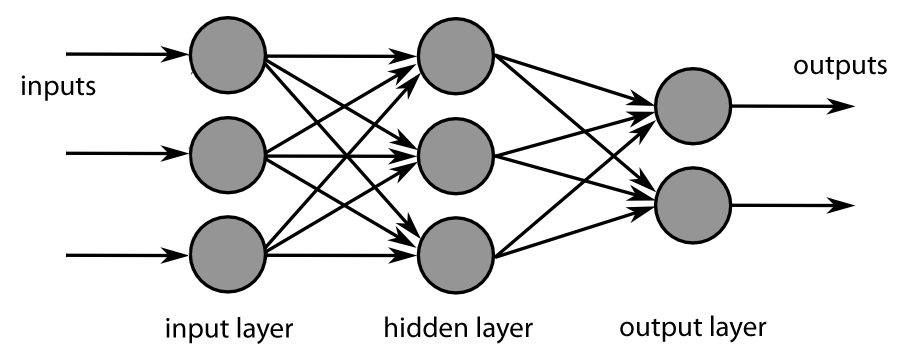
\includegraphics[scale=0.2]{deeplearning}
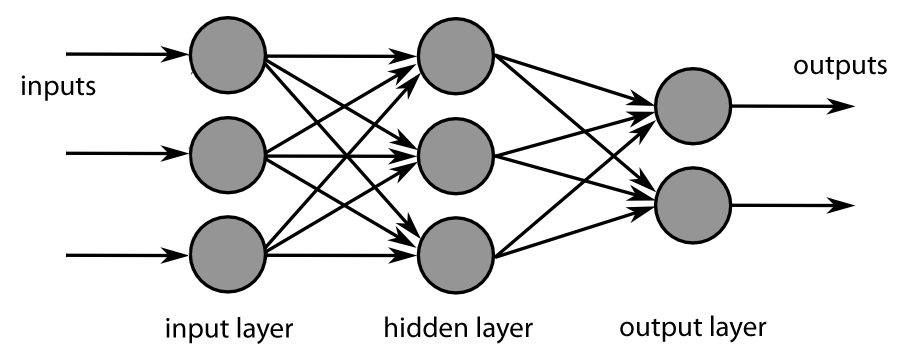
\includegraphics[width=\columnwidth]{deeplearning}
\caption{Beschreibung der Abbildung.}
\label{abbildung1}
\end{figure}

Stet clita kasd gubergren, no sea takimata sanctus est Lorem ipsum dolor sit amet. Lorem ipsum dolor sit amet, consetetur sadipscing elitr, sed diam nonumy eirmod tempor invidunt ut labore et dolore magna aliquyam erat, sed diam voluptua.

\subsection{Überschrift Ebene zwei}

At vero eos et accusam et justo duo dolores et ea rebum. Stet clita kasd gubergren, no sea takimata sanctus est Lorem ipsum dolor sit amet. Lorem ipsum dolor sit amet, consetetur sadipscing elitr, sed diam nonumy eirmod tempor invidunt ut labore et dolore magna aliquyam erat, sed diam voluptua. At vero eos et accusam et justo duo dolores et ea rebum. Stet clita kasd gubergren, no sea takimata sanctus est Lorem ipsum dolor sit amet.

\section{Aufzählungen und Tabellen}

Es folgt eine Aufzählung ohne Nummerierung. Aufzählungen können auch verschachtelt werden.

\begin{itemize}
\item Lorem ipsum
\item dolor sit amet
\item consetetur sadipscing elitr
\item sed diam nonumy
\end{itemize}
Eine nummerierte Aufzählung:

\begin{enumerate}
\item Erster Punkt
\item Zweiter Punkt
\item Dritter Punkt
\end{enumerate}
Es folgt Tabelle \ref{tabelle1}.

\begin{table}[htbp]
\centering
\caption{Beschreibung der Tabelle.}
\label{tabelle1}
\begin{tabular}{lrc}
\toprule
Linksbündig & Rechtsbündig & Zentriert \\
\midrule
Lorem &  13 & amet \\
ipsum & 104 & consetetur \\
dolor &   7 & sadipscing \\
sit   &  -5 & elitr \\
\bottomrule
\end{tabular}
\end{table}

\section{Programmcode}

Programmcode im Fließtext: \lstinline{print("Hello, world!")}.
Lorem ipsum dolor sit amet, consetetur sadipscing elitr, sed diam nonumy eirmod tempor invidunt ut labore et dolore magna aliquyam erat, sed diam voluptua. At vero eos et accusam et justo duo dolores et ea rebum. Stet clita kasd gubergren, no sea takimata sanctus est Lorem ipsum dolor sit amet. Stet clita kasd gubergren, no sea takimata sanctus est Lorem ipsum dolor sit amet. Lorem ipsum dolor sit amet, consetetur sadipscing elitr, sed diam nonumy eirmod tempor invidunt ut labore et dolore magna aliquyam erat, sed diam voluptua. At vero eos et accusam et justo duo dolores et ea rebum.
Es folgt Programmlisting \ref{listing1}.

\begin{lstlisting}[caption={Beschreibung des Listings.}, language=Python, label=listing1, numbers=left, xleftmargin=6mm]
def factorial(x):
    if x <= 1:
        return 1
    return x * factorial(x - 1)
\end{lstlisting}
Ein Listing ohne Titel und Zeilennummern:

% \begin{lstlisting}[language=C]
\begin{lstlisting}
#include <stdio.h>
int main(void)
{
    printf("Hello, world\n");
}
\end{lstlisting}
Text kann zum Beispiel \emph{kursiv} oder \textbf{fett} gesetzt werden.
Lorem ipsum dolor sit amet, consetetur sadipscing elitr, sed diam nonumy eirmod tempor invidunt ut labore et dolore magna aliquyam erat, sed diam voluptua. At vero eos et accusam et justo duo dolores et ea rebum. Stet clita kasd gubergren, no sea takimata sanctus est Lorem ipsum dolor sit amet. Lorem ipsum dolor sit amet, consetetur sadipscing elitr, sed diam nonumy eirmod tempor invidunt ut labore et dolore magna aliquyam erat, sed diam voluptua. At vero eos et accusam et justo duo dolores et ea rebum. Stet clita kasd gubergren, no sea takimata sanctus est Lorem ipsum dolor sit amet.



\printbibliography
\end{document}
